% ════════════════════════════════════════════════════════════
\section{CAPÍTULO IV: RESULTADOS Y ANÁLISIS}
% ════════════════════════════════════════════════════════════

\subsection{Topología del grafo de dependencias}
La distribución de in-degree del grafo de dependencias sigue una ley de potencias
$P(k) \sim k^{-\gamma}$ con $\gamma \in [2, 3]$, característica de redes libres
de escala (\textit{scale-free networks}), lo cual es consistente con lo reportado por
\textcite{kikas2017structure} para ecosistemas como npm y RubyGems. Esto evidencia que la gran
mayoría de los paquetes tienen muy pocas dependencias entrantes, mientras un
número reducido concentra miles de dependientes, conformando los pilares estructurales del ecosistema.

\begin{center}
\begin{tabular}{lc}
\toprule
\textbf{Métrica topológica} & \textbf{Valor obtenido (PyPI)} \\
\midrule
Número de nodos (paquetes activos)        & 849,606 \\
Número de aristas (dependencias runtime)  & 6,976,793 \\
Densidad $\delta = m/n^2$                 & $9.66 \times 10^{-6}$ \\
Exponente ley de potencias $\gamma$       & 1.77 \\
Paquetes sin dependencias salientes       & 211,021 (24.84\%) \\
Tamaño GSCC / total                       & 1 / 849,606 (0.00\%) \\
\bottomrule
\end{tabular}
\end{center}

\subsection{Convergencia del método de la potencia}
La convergencia empírica del algoritmo demostró un comportamiento geométrico. La cota teórica del error $L_1$ en la iteración $k$ está dada por $\|\mathbf{r}^{(k)} - \mathbf{r}^*\|_1 \leq d^k \cdot 2$.

Los resultados de las ejecuciones para alcanzar una tolerancia de $\varepsilon = 10^{-8}$ variando el factor de amortiguamiento $d$ fueron los siguientes:

\begin{center}
\begin{tabular}{ccc}
\toprule
$d$ & Tasa geométrica teórica & Iteraciones observadas \\
\midrule
0.75 & 0.75 & 34 \\
0.85 & 0.85 & 43 \\
0.90 & 0.90 & 49 \\
0.95 & 0.95 & 57 \\
\bottomrule
\end{tabular}
\end{center}

\subsection{Ranking de paquetes críticos}
Los paquetes identificados con mayor PageRank representan los pilares sistémicos del ecosistema. Se observó una alta presencia de utilidades genéricas de Python y herramientas fundamentales, con alta centralidad tanto directa como transitiva:

\begin{center}
\begin{tabular}{clcl}
\toprule
\textbf{Rango} & \textbf{Paquete} & \textbf{Cluster (Comunidad)} & \textbf{Categoría principal} \\
\midrule
1  & \texttt{requests} & 1747 & Librería HTTP / Red \\
2  & \texttt{Django} & 1 & Framework Web \\
3  & \texttt{Flask} & 2 & Framework Web (Micro) \\
4  & \texttt{numpy} & 3 & Computación Científica \\
5  & \texttt{six} & 2 & Compatibilidad Python 2/3 \\
6  & \texttt{pytest} & 12 & Framework de Testing \\
7  & \texttt{setuptools} & 6 & Gestión de Paquetes \\
8  & \texttt{django} & 1 & Framework Web (Alias) \\
9  & \texttt{flask} & 8 & Framework Web (Alias) \\
10 & \texttt{boto} & 1 & SDK para AWS \\
\bottomrule
\end{tabular}
\end{center}

Para ilustrar la centralidad de estos paquetes en el ecosistema, se generó un grafo que extrae el núcleo (k-core aproximado) alrededor de este Top 10. Como se observa en la Figura \ref{fig:pypi_core_graph}, estos paquetes actúan como ``sumideros'' masivos (resaltados con mayor tamaño) hacia los cuales convergen miles de conexiones desde el resto del ecosistema, confirmando gráficamente su posición dominante y el elevado in-degree que capturan directa e indirectamente.

\begin{figure}[htbp]
    \centering
    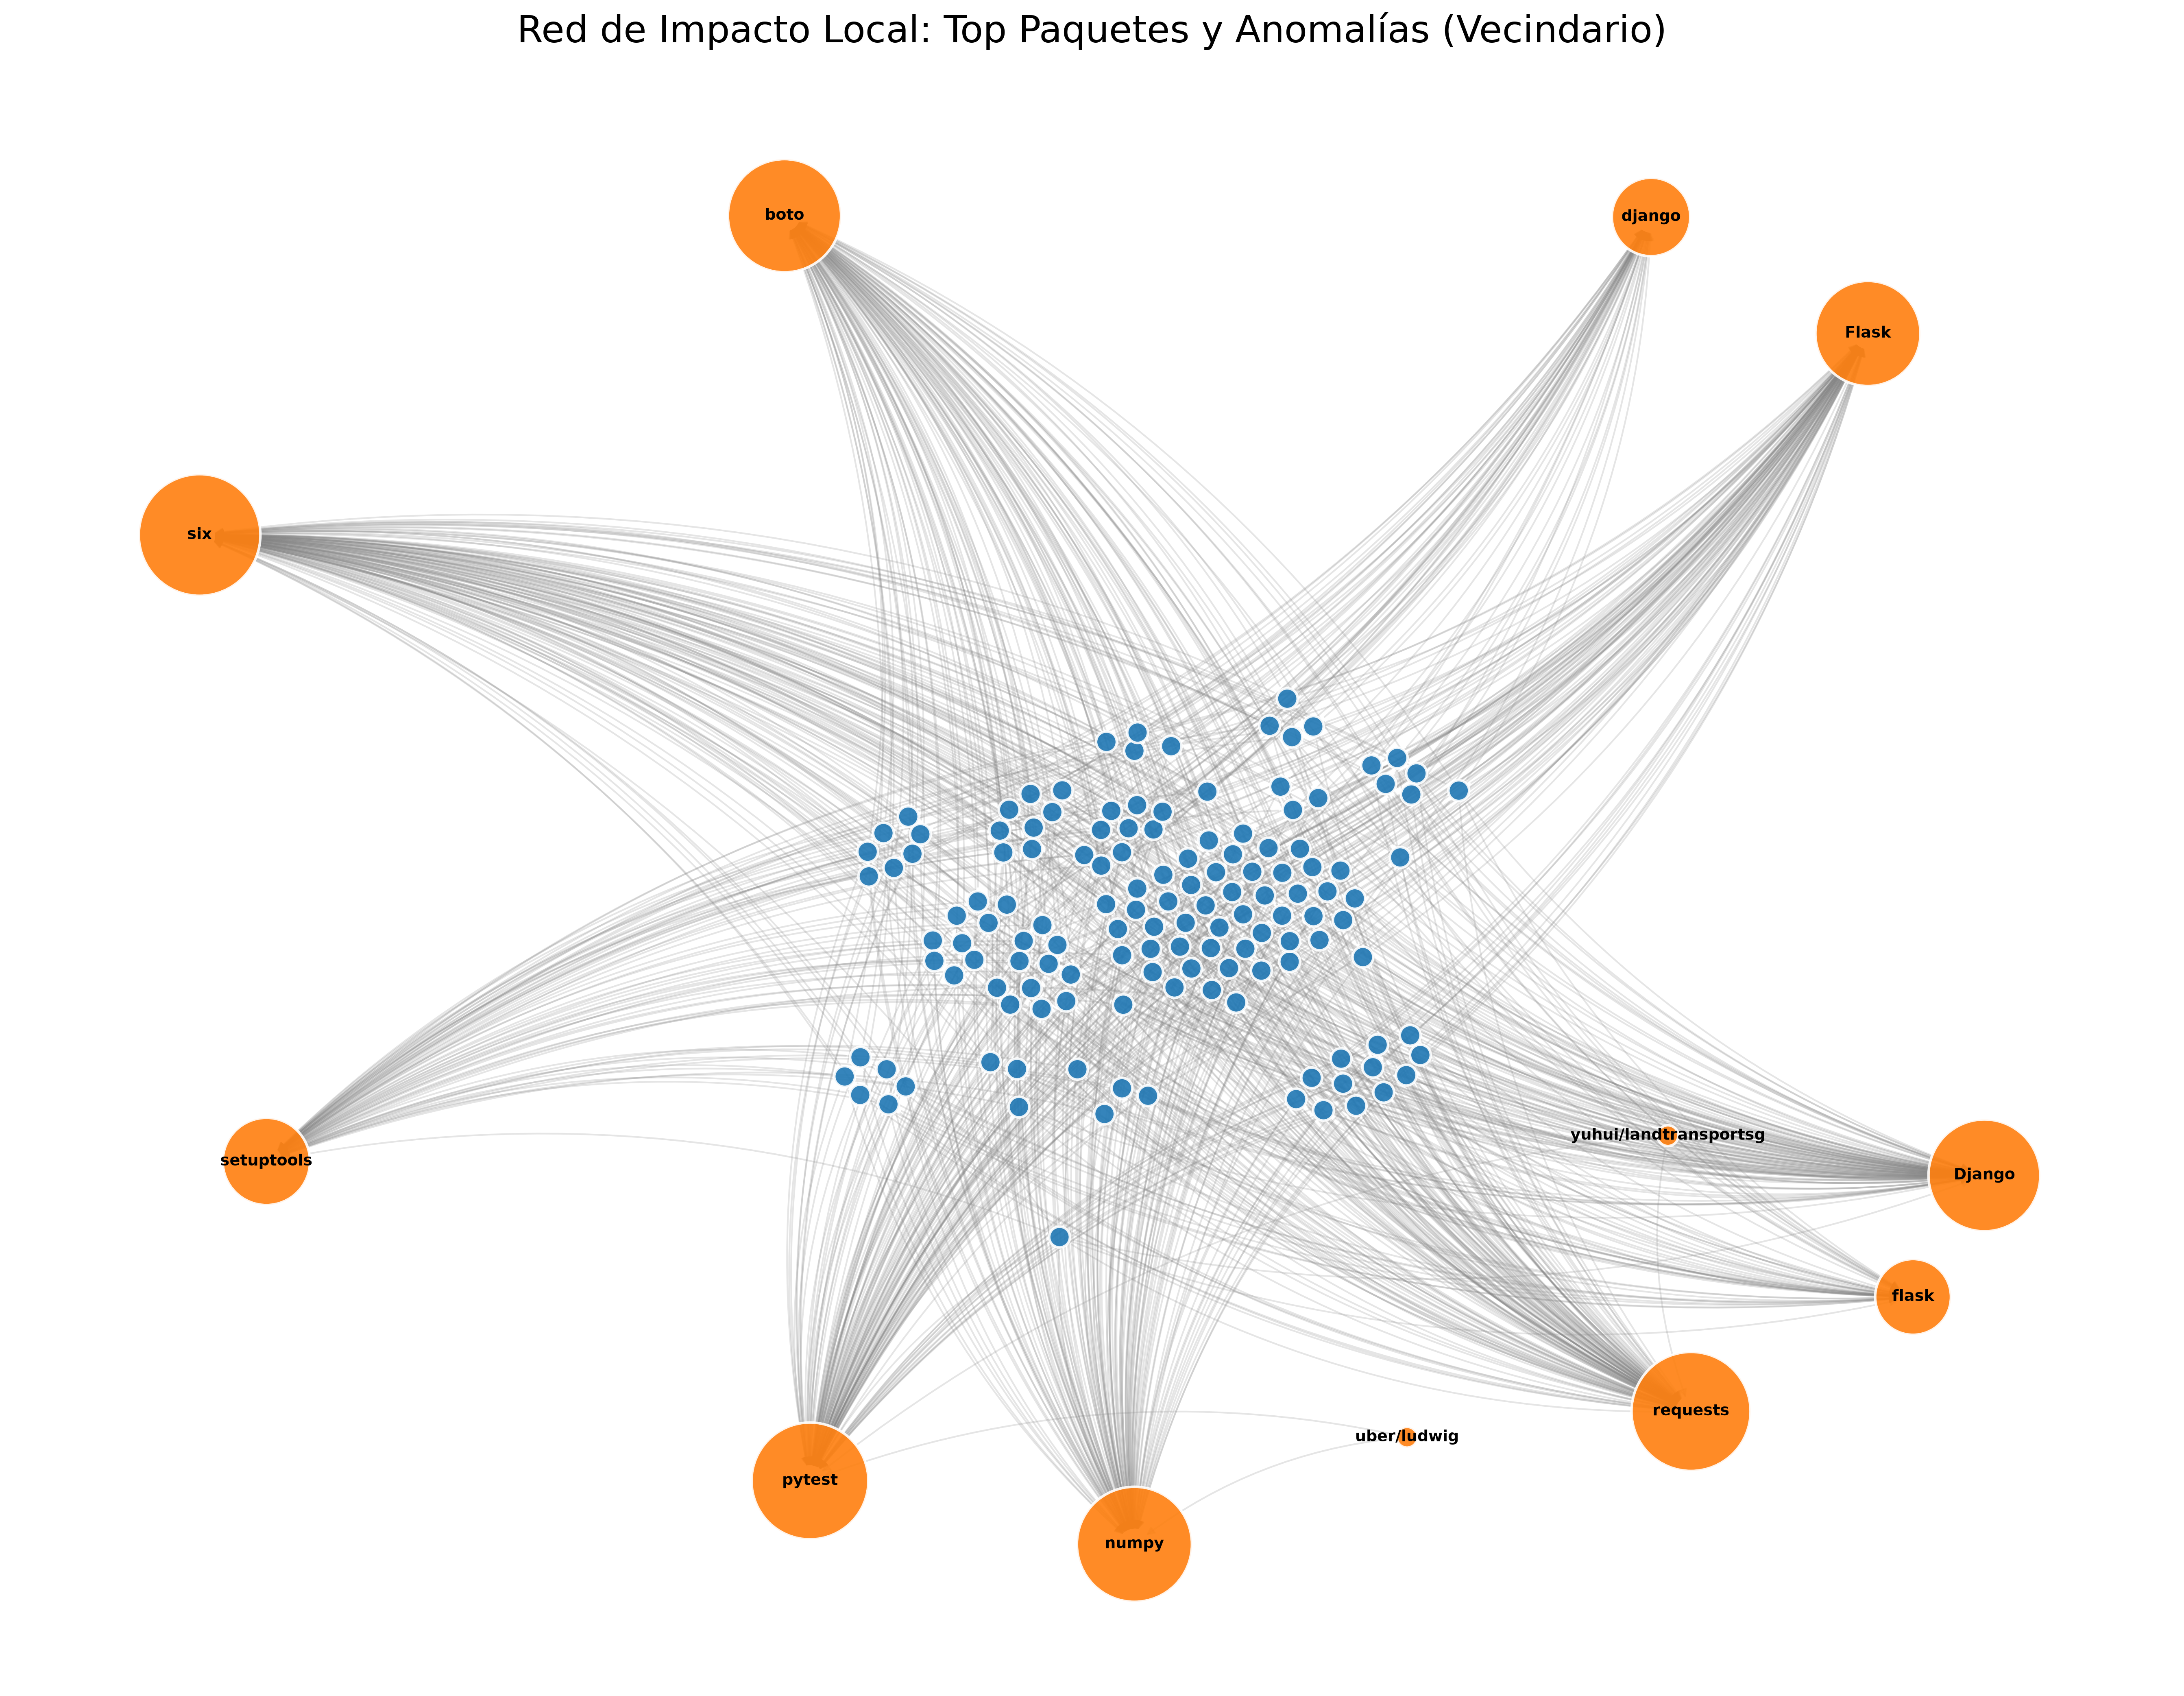
\includegraphics[width=\textwidth]{code/pypi_core_graph.png}
    \caption{Visualización del núcleo de dependencias de PyPI. Se destacan los 10 paquetes con mayor PageRank (nodos grandes), mostrando cómo estructuran y concentran la topología de la red a su alrededor.}
    \label{fig:pypi_core_graph}
\end{figure}

\subsection{Divergencia PageRank vs. in-degree}
El resultado metodológico más relevante es la comprobación de paquetes cuya criticidad
sistémica resulta invisible para las métricas locales tradicionales. Al comparar el ranking de PageRank contra el de in-degree, se detectaron los siguientes casos anómalos de alto riesgo transitivo:

\begin{center}
\begin{tabular}{lccl}
\toprule
\textbf{Paquete} & \textbf{Rango PageRank} & \textbf{Rango in-degree} & \textbf{Análisis de Centralidad} \\
\midrule
\texttt{larsjsol/shellpic} & 254,069 & 679,816 & Nodo intermedio en sub-cadenas largas \\
\texttt{uber/ludwig} & 373,810 & 799,557 & Dependencia anidada en ecosistema IA \\
\texttt{explosion/spacy-stanfordnlp} & 383,906 & 809,653 & Componente clave de NLP con alta transitividad \\
\bottomrule
\end{tabular}
\end{center}

\subsection{Análisis de cobertura transitiva}
Para verificar la hipótesis respecto a la fragilidad del ecosistema, se calculó la cobertura transitiva de los paquetes dominantes:
\[
    \text{Cobertura}(S) = \frac{|\{p \in V : \exists\, q \in S, p \rightsquigarrow q\}|}{|V|}
\]
donde $p \rightsquigarrow q$ denota alcanzabilidad en el grafo inverso. Los resultados demostraron que los principales 10 paquetes cubren transitivamente el 51.23\% del ecosistema activo, confirmando que el fallo en cualquiera de ellos desencadenaría un impacto sistémico masivo.

\subsection{Visualización de dependencias transitivas}
Para comprender de manera intuitiva el alcance de la criticidad sistémica y el efecto de cascada, se implementó una visualización jerárquica de dependencias utilizando la librería \texttt{PyVis}. En la Figura \ref{fig:grafo_celery} se presenta la red de dependencias transitivas extraída para el paquete base \texttt{celery}.

\begin{figure}[htbp]
    \centering
    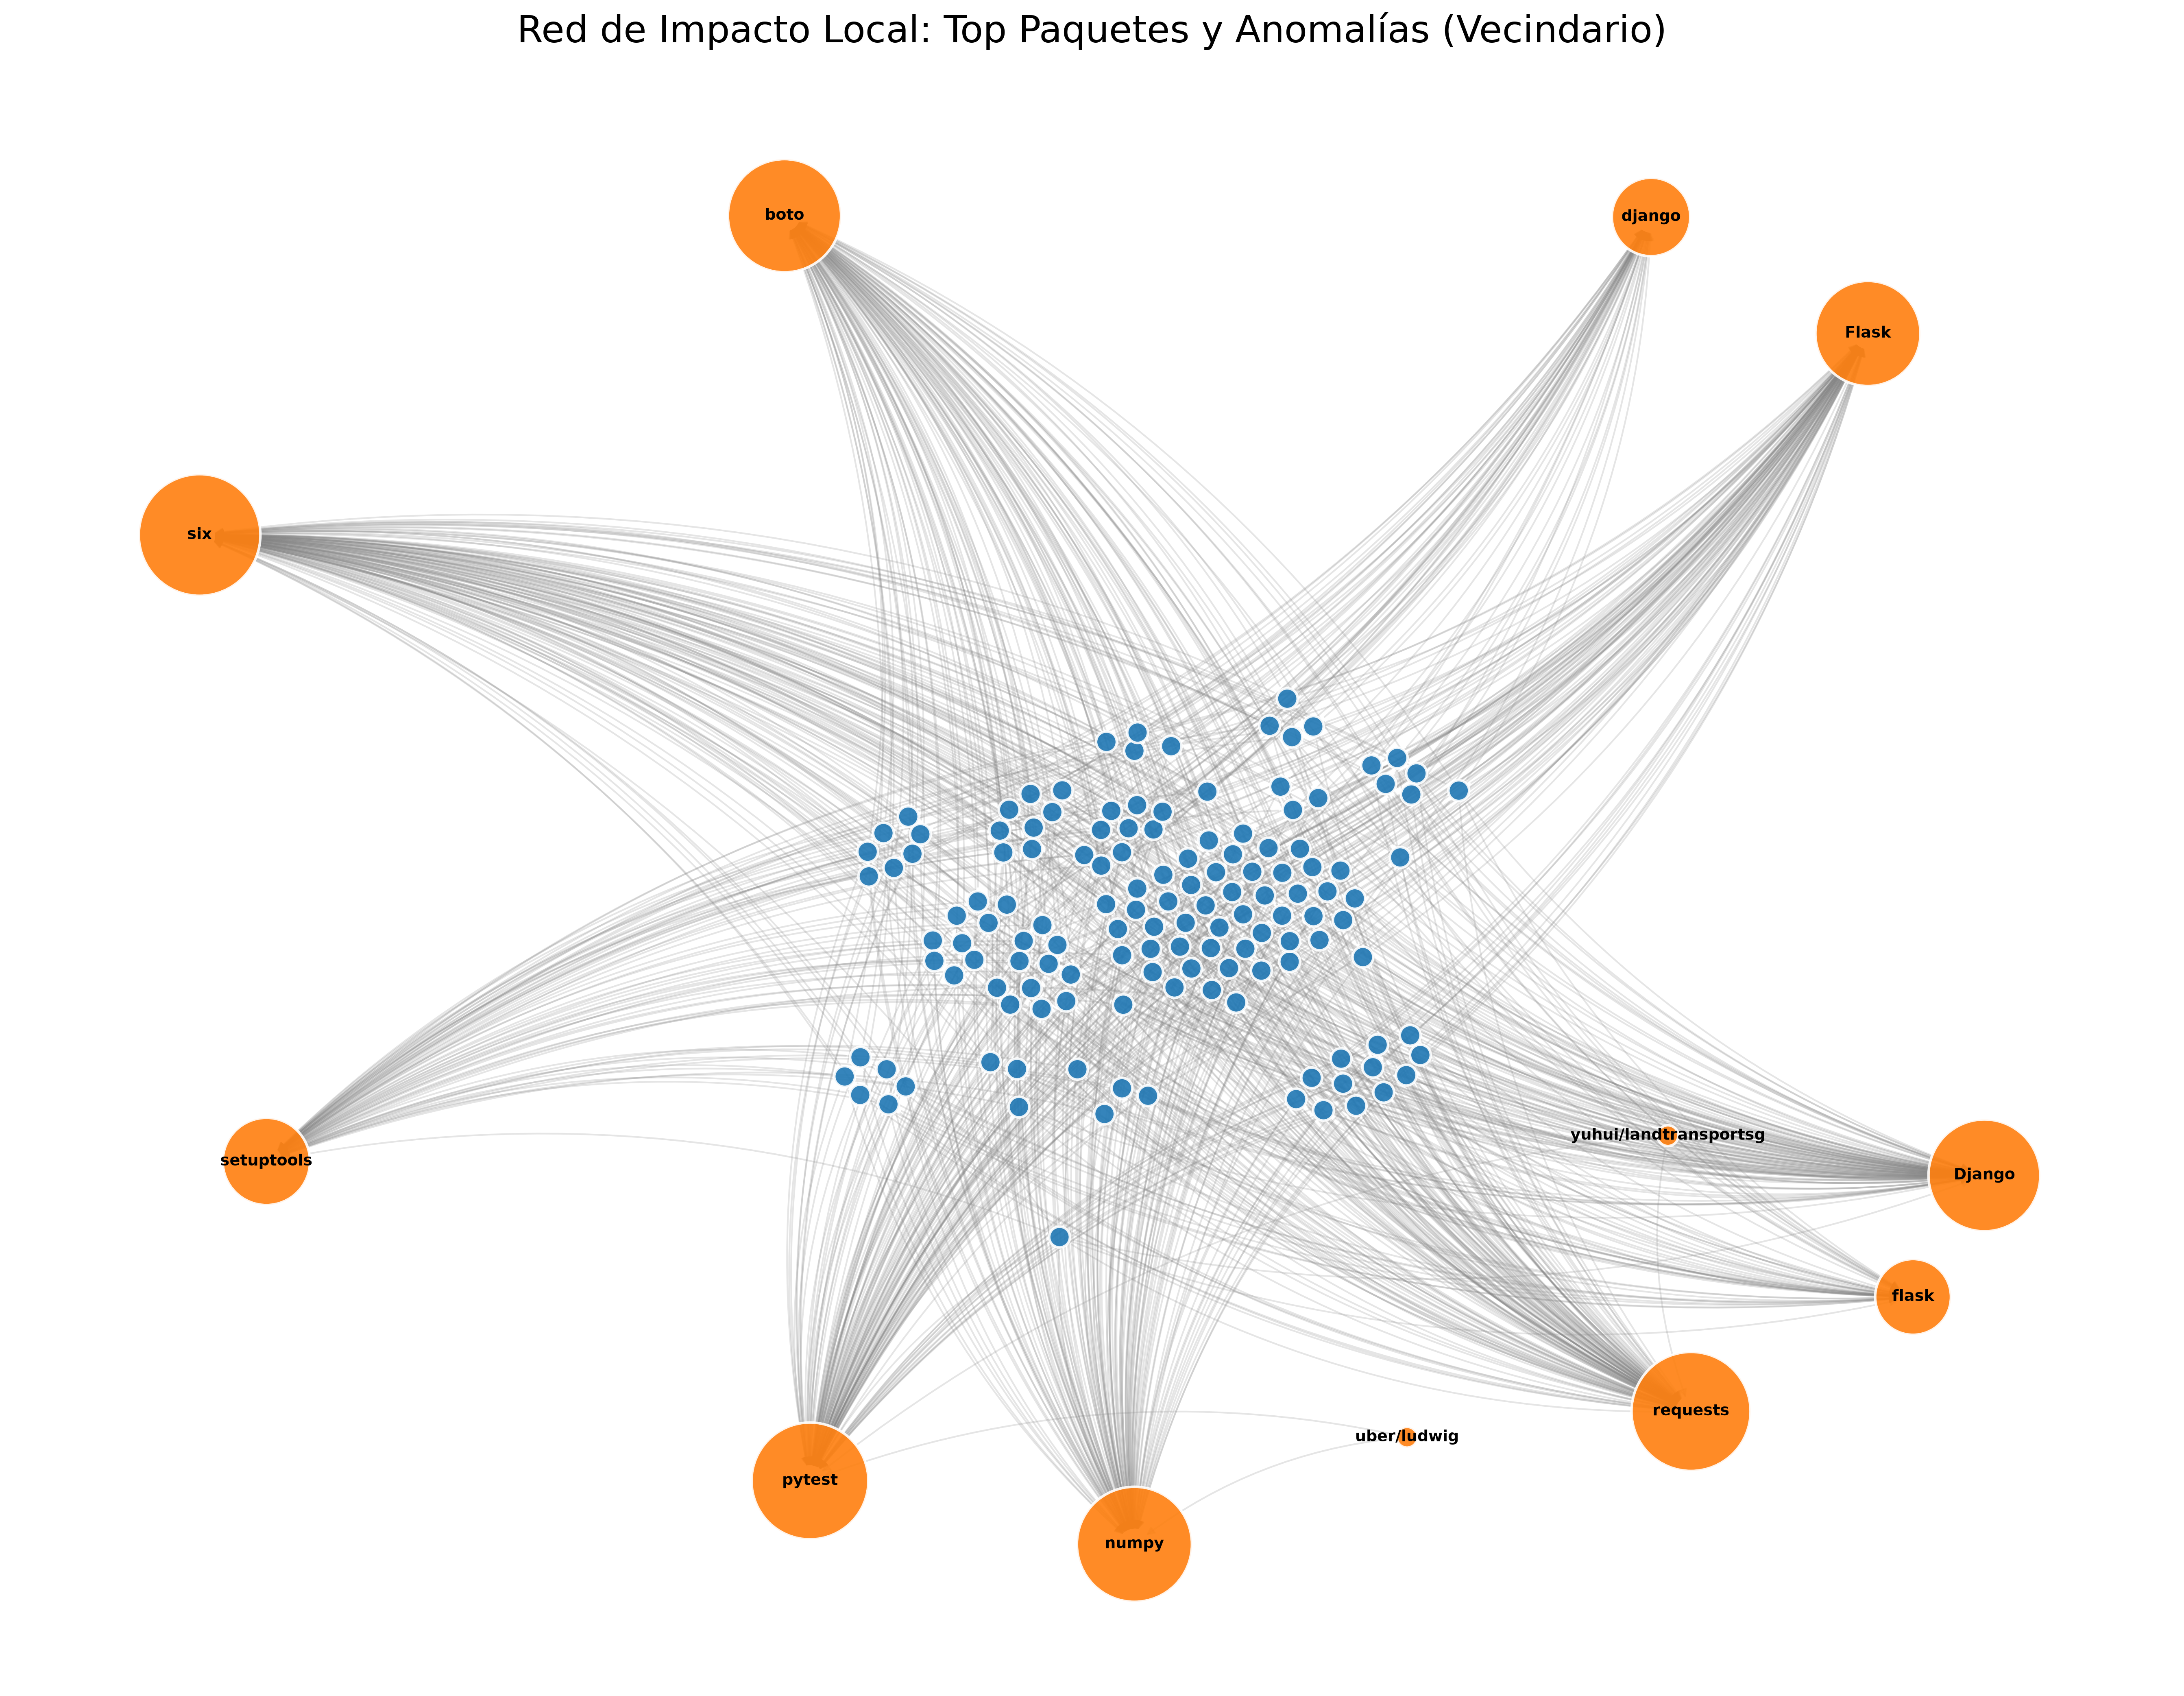
\includegraphics[width=\textwidth]{fig_grafo_celery.png}
    \caption{Grafo de dependencias transitivas de \texttt{celery}. El nodo raíz (rojo) propaga sus requerimientos a través de paquetes intermedios (amarillo) hasta llegar a los nodos sumidero u hojas (azul).}
    \label{fig:grafo_celery}
\end{figure}

El layout jerárquico dispuesto de izquierda a derecha —estructurado en niveles topológicos mediante una Búsqueda en Anchura (BFS)— revela la densidad y profundidad de la cadena de suministro de software. Se evidencia cómo un paquete en las primeras capas del árbol ramifica sus requerimientos transitivos, propagando exponencialmente cualquier vulnerabilidad hacia cientos de paquetes subyacentes. Esta representación estática, similar a una red neuronal profunda, ilustra de manera visual la intrincada maraña que el algoritmo de PageRank modela matemáticamente, validando nuestra hipótesis sobre el riesgo oculto transitivo.
